\pdfoutput=1

\documentclass{article}
\usepackage{fullpage}
\usepackage{amsmath,amssymb,amsfonts}
\usepackage{bm}
%\usepackage{bbm}
%\usepackage{tikz}
%\usepackage[normalem]{ulem}
%\usepackage{hhline}
\usepackage{graphicx}
\usepackage{subfig}

\graphicspath{{./figs/}}

\usepackage{color}
%\usepackage{doi}

%\renewcommand{\topfraction}{0.85}
%\renewcommand{\textfraction}{0.1}
%\renewcommand{\floatpagefraction}{0.75}
%
%
%\newcommand{\bbm}[1]{\mathbbm{#1}}
%\newcommand{\bs}[1]{\boldsymbol{#1}}
%\newcommand{\equaldef}{\stackrel{\mathrm{def}}{=}}
%
%
%\newcommand{\mb}[1]{\mathbf{#1}}
%\newcommand{\mbb}[1]{\mathbb{#1}}
%\newcommand{\mc}[1]{\mathcal{#1}}
%
%\renewcommand{\hat}{\widehat}
%\renewcommand{\tilde}{\widetilde}
\newcommand{\td}[2]{\frac{{\rm d}#1}{{\rm d}{\rm #2}}}
\newcommand{\pd}[2]{\frac{\partial#1}{\partial#2}}
%\newcommand{\pdn}[3]{\frac{\partial^{#3}#1}{\partial#2^{#3}}}
%\newcommand{\snor}[1]{\left| #1 \right|}
%\newcommand{\nor}[1]{\left\| #1 \right\|}
\newcommand{\LRp}[1]{\left( #1 \right)}
\newcommand{\LRs}[1]{\left[ #1 \right]}
%\newcommand{\LRa}[1]{\left\langle #1 \right\rangle}
%\newcommand{\LRb}[1]{\left| #1 \right|}
%\newcommand{\LRc}[1]{\left\{ #1 \right\}}
%\newcommand{\LRceil}[1]{\left\lceil #1 \right\rceil}
\newcommand{\LRl}[1]{\left. \LRp{#1} \right|}
\newcommand{\nor}[1]{\left\|#1\right\|}
%\newcommand{\jump}[1] {\ensuremath{\llbracket#1\rrbracket}}
%\newcommand{\avg}[1] {\ensuremath{\LRc{\!\{#1\}\!}}}
%\newcommand{\Grad} {\ensuremath{\nabla}}
%\renewcommand{\d}{\partial}
\newcommand{\diag}[1]{{\rm diag}\LRp{#1}}

\newcommand{\note}[1]{{\color{blue}{#1}}}
\newcommand{\bnote}[1]{{\color{blue}{#1}}}
\newcommand{\rnote}[1]{{\color{red}{#1}}}


\newcommand{\LK}{L^2\LRp{D^k}}
\newcommand{\LdK}{L^2\LRp{\partial D^k}}
\newcommand{\Dhat}{\widehat{D}}
\newcommand{\Lhat}{L^2\LRp{\Dhat}}


\newcommand*\diff[1]{\mathop{}\!{\mathrm{d}#1}} % d in integrand



\begin{document}

%\maketitle

\note{We thank the two Reviewers for their feedback, and describe steps taken to address reviewer comments and suggestions in the following response.  We have also addressed the typos described in the minor comments by each reviewer.  For brevity, we have not included typo and minor comment responses in this response.
\\
\\
Revisions in the manuscript are also colored for ease of identification.  We hope these revisions improve the readability of this paper and its suitability for the audience of SISC.}

\section{Reviewer 2}

We thank reviewer 2 for their careful reading of the paper.  In particular, we are grateful for the minor comments provided, which fixed several small typos and errors in the submitted manuscript.

\begin{itemize}
\item In equation (2), the entropy potential $\psi_i(u)$ is used but never defined. I also noticed that while the entropy function $S(u)$ is mentioned, the corresponding entropy flux is never mentioned. Is this intentional?  

\bnote{We thank the reviewer for pointing this out.  We have added a definition of $\psi_i(u)$ after equation (2).  The reviewer is also correct that we intentionally do not mention the entropy flux.  This is because it factors into the continuous derivation of an entropy inequality, but not in the discrete derivation.  In the continuous derivation, the entropy flux factors into the entropy inequality via the chain rule, which does not hold discretely. }

\item In equation (7), a $\Delta x$ term seems to be missing before $\bm{K}\bm{u}_h$. Furthermore, since the viscous term is a discrete version of the Laplacian with periodic boundary conditions, it is a bit strange that the first and last rows of K seem to represent the discretization of the second order derivative when Neumann/open boundary conditions are considered. Could the author comment on this?

\bnote{We thank the reviewer for pointing this out, and have fixed it in the revision.  We have also clarified that the choice of Neumann boundary conditions is arbitrary, and can be replaced with the periodic Laplacian.  However, we have not noticed a significant difference in numerical experiments between the use of periodic boundary conditions and open/Neumann boundary conditions for the Laplacian.  We adopt Neumann boundary conditions for all experiments because they appear to work for both periodic and reflective wall boundary conditions.  
\\
\\
Future works will investigate different viscous boundary conditions (such as solid wall conditions) and their impacts on reduced order models.
}

\item  In the first line after Assumption 1 on page 8, the author states that ”the column space of $V$ is contained in the column space of $V_t$”. However, no connection between these two spaces has been made up to this point. I presume this is true because of the way $V_t$ is constructed, which is mentioned much later in the text. I would recommend minor rearrangements to make this fact clearer.

\bnote{We thank the reviewer for pointing this out.  We have added a statement on the previous page when $\bm{V}_t$ is introduced stating that ``In this work, we assume that the span of the test basis includes the reduced basis, e.g., $\mathcal{R}(\bm{V})\subset \mathcal{R}(\bm{V}_t)$.''}

\item  In the proof for Lemma 2, it was not clear to me how $\mathcal{R}(QV) \subset \mathcal{R}(V_t)$ implies $e_2 \in \mathcal{R}(V_t)$. Could the author explain this? If it is straightforward, it need not be added to the proof.  

\bnote{We thank the reviewer for catching this - it was an error on our part.  We have replaced the lemma with another discussion of how the choice of test space affects accuracy.  }
%\bnote{Certainly.  $\bm{e}_2$ is the linear combination of $\bm{Q}{\bm{V}_t\bm{V}_t^{\dagger}}\bm{f}$ and $\LRp{\bm{V}_t\bm{V}_t^{\dagger}}^T\bm{Q}\bm{V}_t\bm{V}_t^{\dagger}\bm{f}$.  The first term $\bm{Q}{\bm{V}_t\bm{V}_t^{\dagger}}\bm{f}$ is $\bm{Q}$ applied to some vector, so the result is in the range of $\bm{Q}$ (and thus in the range of $\bm{V}_t$ by the assumption).  The latter term is $\LRp{\bm{V}_t\bm{V}_t^{\dagger}}^T$ multiplied by some vector, and since $\bm{V}_t\bm{V}_t^{\dagger}$ is a symmetric projection matrix, the latter term is in the range of $\bm{V}_t$.  } 


\item In Algorithm 1, what is the advantage of performing a linear least square approximation for $w$, followed by a non-negative least squares if a negative weight is obtained?  Why not directly use non-negative least squares to begin with?

\bnote{This approach follows the approach taken in \cite{hernandez2017dimensional}, where they noted that for many test cases, the non-negative least squares (NNLS) solve was not necessary to guarantee positivity of weights.  Replacing the NNLS solve with a standard least squares solve ended up being noticably less expensive.  }

\item In Section 4.3, additional stabilization points are added to ensure that the test mass matrix is non-singular. But is it guaranteed that this approach used will always lead to such a matrix?

\bnote{We thank the reviewer for bringing up this question.  Because the algorithm is greedy, it will continue to add points so long as the test mass matrix is near singular, so the test mass matrix will eventually end up being non-singular (in the limiting case, the algorithm will simply choose all FOM points).  However, it is unclear how many points need to be added to avoid near-singularity.  The choice of $\alpha$ and use of the near-null space of the test mass matrix are thus heuristic approaches to reduce how many stabilizing points we need to add. }

\item In Section 4.5, the author mentions tricks to improve the computational costs when polynomial-type function are considered. However, the entropy conservative fluxes used for the Euler equations makes use of logarithmic terms. Then would such tricks be helpful in the context of the experiments presented in this manuscript?

\bnote{They unfortunately would not be helpful for the experiments in this work, at least not without giving up discrete entropy conservation (dissipation).  We have added a footnote explaining this:
\\
\\
``Because entropy conservative fluxes for the compressible Euler equations include non-polynomial rational and logarithmic terms, it is not possible to apply this exact treatment of polynomial nonlinearities to general entropy conservative discretizations.''}

\item The expression for the entropy variable on page 20 all seem off by a factor of $(\gamma -1)$ compared with the expressions in the paper by Chandrashekar [66]. My guess is that the expression in this manuscript may be correct for the choice of the entropy function $S(u) = -\rho s$. Could the author verify this?

\bnote{We thank the reviewer for catching this.  We have corrected the entropy function in the revised manuscript.}

\item What was the value of $\epsilon$ for the experiments shown in Figure 3. Furthermore, what is the difference between running the model in the absence of viscosity and running the model by setting $\epsilon = 0$, as mentioned in the first paragraph on page 22?

\bnote{We have added $\epsilon = 2e-4$ to the description.  We have also removed the sentence with $\epsilon = 0$, which the reviewer has correctly pointed out is redundant.}

\item To truly judge the benefits of using ROMs, it would be useful if the actual computational times for the full model, and the time for the offline+online computation of the ROM is provided for at least one of the 2D experiments. 

\bnote{We agree with the reviewer's comments, but note that for the 2D problems considered, the proposed entropy stable reduced order models are more expensive than the full order model due to the use of explicit time-stepping.  This is described some in the conclusion of the original submission, but we have significantly expanded the discussion in the revised paper in a new section (see Section 7.3).  The discussion is quoted below:
\\
\\
\textit{We note that the entropy stable reduced order models implemented in this work do not reduce computational cost compared to the original full order models due to the use of explicit time-stepping.  Explicit time-stepping is used in this paper to validate the proposed semi-discrete formulation.  However, we expect that for implicit time-stepping, entropy stable ROMs will see more significant efficiency gains.  
\\
\\
The cost of explicit time-stepping schemes scales with the cost of the ODE right hand side evaluation, and the cost of a right hand side evaluation for an entropy stable scheme scales with the number of entropy conservative flux evaluations required.  The number of entropy conservative flux evaluations is the same as the number of nonzero entries in the matrix $\bm{Q}^i$, since the nonlinear term is $\LRp{\bm{Q}^i\circ\bm{F}^i}\bm{1}$ and the entries of the matrix $\bm{F}^i$ (which are flux evaluations between different states) are evaluated on the fly.  
\\
\\
For the 2D full order methods in this paper, the differentiation matrices $\bm{Q}^i$ are sparse with $O(K^2)$ non-zero entries.  Thus, the cost of a 2D entropy stable finite volume method is $O(K^2)$ nonlinear flux evaluations for each coordinate direction.  For a reduced order model, however, the hyper-reduced matrices $\bm{Q}^i_t$ are dense, and evaluating $(\bm{Q}^i_t \circ \bm{F}^i)\bm{1}$  requires $O(N_s^2)$ flux evaluations where $N_s$ is the number of hyper-reduced points.  As an example, consider the Kelvin-Helmholtz results in Figure~8.  The full order model requires $O(40000)$ flux evaluations.  However, because the ROM has $884$ hyper-reduced points, $O(781,456)$ flux evaluations are required, resulting in a ROM which is more expensive per time-step than the full order model.  
\\
\\
While the proposed ROMs could still provide savings for sufficiently large full order models, this increased cost is a significant issue for explicit time-stepping.  The cost is offset slightly if the ROM has a larger CFL \cite{marley2015reduced}; however, this situation only occurs if a smaller number of modes are used to simulate the solution.  The situation changes for implicit time-stepping, as full order models require multiple solutions of large (but sparse) linear systems at each time-step.  For a $K\times K$ grid, these linear systems would require $O(K^2)$ flux evaluations to assemble, but we expect the solution of the linear system to be the dominant cost.  For a ROM using implicit time-stepping, the assembly of the linear system still requires $O(N_s^2)$ flux evaluations, but the size of the system scales with the number of modes, which is notably smaller than even the number of hyper-reduced points.  For example, the Kelvin-Helmholtz example uses only $75$ basis functions per component, compared to $884$ hyper-reduced points.  We thus expect that the use of entropy stable ROMs will result in a more significant speedup under implicit time-stepping.
}
}
\item It would be interesting to see how the proposed ROM works for a more complex 2D problem. Perhaps the author could also test with a 2D Riemann problem for the Euler equations where shocks and/or contact discontinuities interact with each other. If discontinuous initial conditions is a problem, the author could choose a smooth approximation connecting the 4 states.

\bnote{
We have included the results from a smoothed 2D Riemann problem simulation in this reviewer response (see Figure~\ref{fig:riemann}).  The problem is taken from \cite{chan2017discretely}, and is modified to use periodic boundary conditions (due to the fact that ``natural'' boundary conditions are not provably entropy stable).  The FOM is run until time $T=.25$ on a $200\times 200$ grid with a CFL of $.25$ and $\epsilon = 5e-3$.  The ROM uses $50$ modes and $812$ hyper-reduced points, and achieves a final $L^2$ error of $0.03278$.  The ROM runs stably despite the presence of oscillations along the shock traveling to the north-east.  The solution appears reasonably well-approximated in smoother areas.
\\
\\
We would like to run this experiment with a larger number of modes to ensure that the ROM solution converges to the FOM.  However, because our implementation for these early experiments is not well-optimized, the hyper-reduction step becomes very slow as the number of modes increases.  For this reason, we have not included the example in the paper, but would be happy to do so if the reviewer believes this will improve the quality of the paper.
}
\begin{figure}
\centering
\subfloat[FOM results]{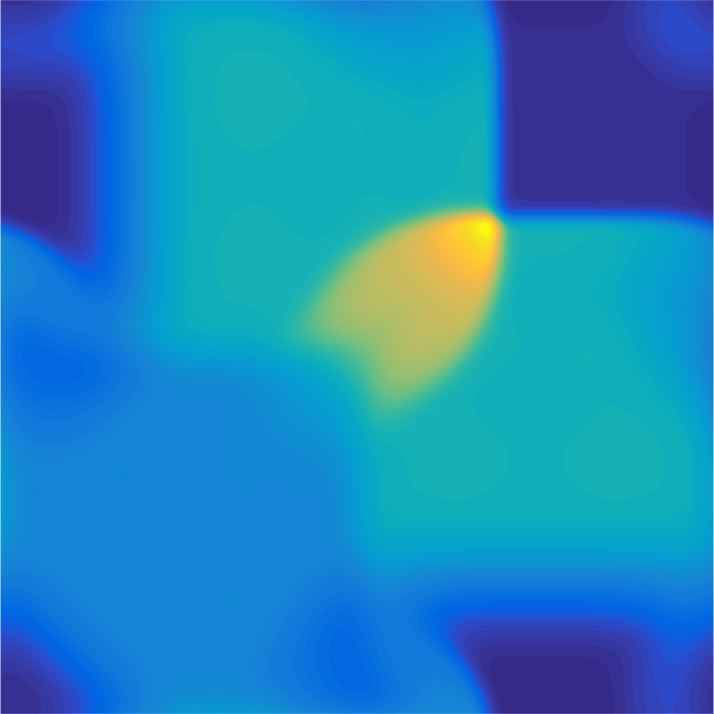
\includegraphics[width=.3\textwidth]{riemannFOM.png}}
\hspace{.25em}
\subfloat[ROM results]{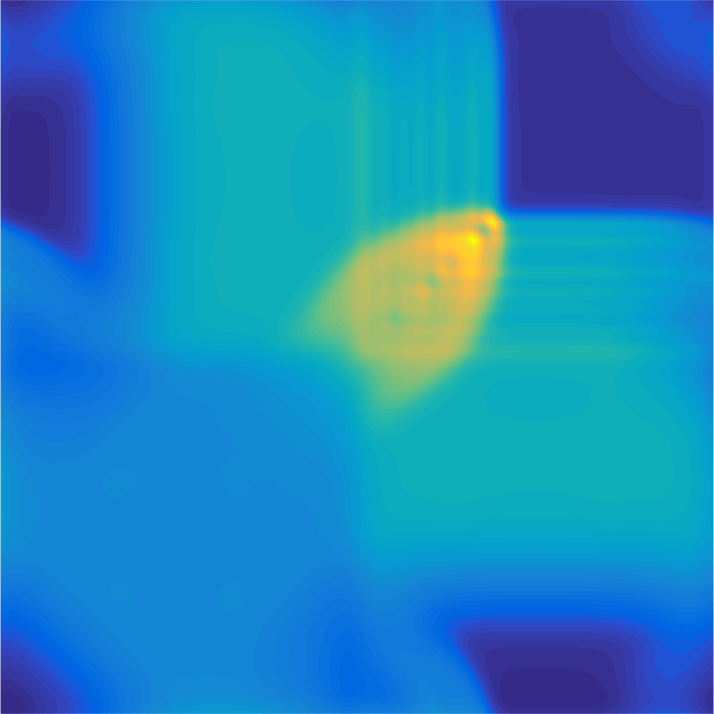
\includegraphics[width=.3\textwidth]{riemannROM.png}}
\hspace{.25em}
\subfloat[Hyper-reduced points]{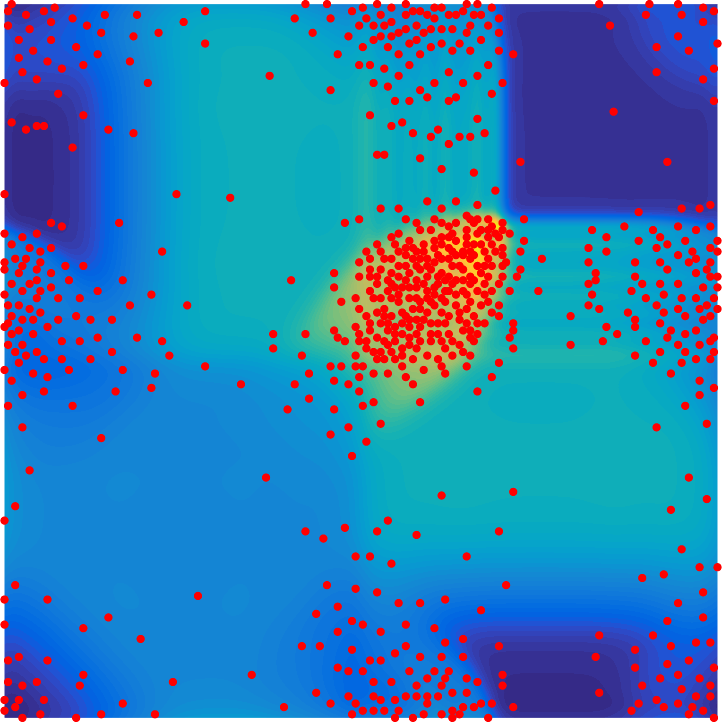
\includegraphics[width=.3\textwidth]{riemannROM_hrpts.png}}
\caption{Comparison of ROM and FOM behavior for a 2D Riemann problem.}
\label{fig:riemann}
\end{figure}

\item In the expressions for the viscous terms in Section 4.6, the viscosity coefficient seems to be missing. Or rather, it has been implicitly taken as unity. Is this intentional?  Is the viscous term in equation (19) missing a $V^T$?  

\bnote{We thank the reviewer for catching these issues.  The reviewer is correct that these are typos, and we have fixed this in the revised paper.}

\end{itemize}

\section{Reviewer 3}

We thank reviewer 2 for their feedback on the submitted paper, and for bringing up issues facing reduced basis approximations of transport-dominated problems.

\begin{itemize}
\item My main question is the following: the author construct a POD decomposition using shnapshots as usual. What I do not understand is why this POD basis should be good for long term unsteady solution. I am talking about section 3 where everything is done at the semi-discrete level, so time is missing.  

Assume that one shock appears, then I guess that the POD data base should take into account this. However, if the data base is constructed with many parameters, there is no reason why apriori one should know if there will be shocks or not, so how do you proceed in practice. What are the limitations?
I have the same question for unsteady problem in general: if you take
$u_t+u_x =0$ on $[0,1]$ with inflow conditions, and $u(x,0)=$ heaviside, then the number of POD is approximately the number of grid points.

Here on the contrary, you need few modes. is it because of the structure of your problems (for example the Burgers one has a symmetry as you mention), or of the numerical dissipation you are adding (but does it solve the advection problem)???  There is nothing in the text that helps understanding why this works.


\rnote{We thank the reviewer for pointing this out, and agree that the POD basis is not ideal for transport-dominated problems.  However, POD based approaches can still be used in the model reduction of transport-type equations so long as the solution retains some structure (either symmetry in the Burgers' example, or a quasi-periodic structure for the captive-carry problem in \cite{carlberg2013gnat}).  These approaches are not optimal, but are still useful to some practitioners.  To clarify these points, we have added a paragraph to the introduction describing these approximation challenges.  
\\
\\
``We note that this work focuses on classical model reduction techniques, which lose effectiveness for general transport-type phenomena \cite{reiss2018shifted, abgrall2018model, rim2018transport, cagniart2019model}.  This is tied to difficulties in approximating convected solutions using a fixed reduced basis.  Despite these challenges, classical approaches are still in model reduction of transport-type equations for specific problem setups \cite{carlberg2013gnat}.  In this work, we restrict ourselves to classical model reduction techniques.  Challenges associated with the low-dimensional approximation of transport-type solutions will be addressed in future work.'' }


\item In section 4, you should give more details. For example the paragraph starting with "weigts in section 4.2" till just before the section 4.1 is really sketchy.

\rnote{We apologize for the confusion in this paragraph.  We have re-written it in the revised version.  In particular, we have added the following paragraph to outline our approach to hyper-reduction:
\\
\\
''We briefly outline our approach to hyper-reduction.  Rather than directly apply hyper-reduction on the nonlinear vector, we perform a matrix-based hyper-reduction which respects the matrix structure of the nonlinear term $\bm{V}^T\LRp{\bm{Q}\circ \bm{F}}$.  Specifically, we construct a smaller hyper-reduced matrix $\bm{Q}_s$ and approximate the term $\bm{V}^T\LRp{\bm{Q}\circ \bm{F}}$ with $\bm{V}\LRp{\mathcal{I},:}^T\bm{W}\LRp{\bm{Q}_s\circ \bm{F}_s}$, where $\bm{F}_s$ is a smaller hyper-reduced matrix containing flux evaluations between solution states at different hyper-reduced points.''
\\
\\
Additional changes were also made to clarify this paragraph. }

\item In 4.1, how do you ensure in practice the assumption 1?

\rnote{We have added a sentence explaining that a heuristic algorithm for ensuring Assumption 1 is provided in a later section (Section 4.3).}

\item What is new in lemma 2: if $A$ is a linear operator, we all know that $||Ax-Ay|| \leq ||A||  ||x-y||$.  Since I imagine that you want to say something different, maybe the formulation should be changed.  In fact you confuse the reader: you show one thing $Qf-(VV^\dag)^TQ(VV^\dag) f=Q(f-(VV^\dag) f )$, then the inequality is trivial.

\rnote{We thank the reviewer for pointing this out.  We have replaced the lemma (which also contained an error) with a simpler discussion of why the choice of test space reproduces the action of $\bm{Q}$ on the reduced basis matrix $\bm{V}$.  }

\item In 4.2, hyper reduction, I do not see/understand how you take into account the time: are the hyperreduced modes good for ever, and why, or not ? what are the limits of the method.  

\rnote{We have added two sentences to clarify this point.  In Section 3, we specify that ``We assume that the solution is well-approximated in the reduced basis over the entire time-window of the simulation''.  
\\
\\
In Section 4.2, we have added ``Because we assume a fixed reduced basis in time, we compute a single set of empirical cubature points prior to the simulation and use those same points over the entire duration of the simulation''.  We also suggest approaches which can be combined with our proposed methodology to address this challenge in future work.  Section 4.2 includes the sentence ``Again, we emphasize that solution snapshots for transport-type equations may not be well-approximated by a low-dimensional reduced basis.  Future work will attempt to combine techniques introduced in this work with methods to address this approximation issue \cite{reiss2018shifted, rim2018transport, cagniart2019model}.''
}

\item page 22 you write ``We now compare the evolution of both the L2 error and discrete entropy,'' the L2 error of what?

\rnote{We have clarified that this is the discrete $L^2$ error between all components of the full and reduced order solutions. }

\item One things that makes me a bit confused: if I understand well, the norm that you use for the POD is related to the entropy (so again  my question about time). and many times in the text, you talk about L2 norm, is it the one related to the entropy, for example $\int_0^T <x, A_0 x> dx$, where $A_0$ is the Hessian of the entropy evaluated at $U(.,t)$, or something else, and what.

\rnote{We have added the following sentence clarifying the definition of the $L^2$ norm: ``Here, the discrete $L^2$ norm is defined as $\nor{\bm{u}}^2 = \Delta x^2 \bm{u}^T\bm{u}$ in 1D or $\nor{\bm{u}}^2 = (\Delta x \Delta y)^2 \bm{u}^T\bm{u}$ in 2D, and is the analogue of the continuous $L^2$ norm evaluated at discretization points for the full order model.''}


\item your description of the finite difference scheme, with Hadamard product, is not very classical in the hyperbolic community. I am not saying it is wrong, I say it is not conventional. So the reading starts to be hard after page 3, in the sense we need a dictionary. This should improved.

\rnote{We thank the reviewer for pointing this out.  We have added some sentences which try to point out non-standard notation, and try to provide some references to papers where a similar notation is used.  For example, on page 3, we have added the sentence ``We note that this reformulation using the Hadamard product is non-standard within the finite volume literature, but is more common in the SBP finite difference literature.''}

\item page 5, formula 2, before (9): you should write you use a path to compute the average Jacobian, and do it componentwise, other wise it does not make much sens.  take  (classical counter example) $f(x)=e^{i\pi x}, f(1)-f(0)=-2, f'(x)=i\pi f(x) and -2 =i\pi f(\xi) * (1-0)$ is not possible because $|-2|=2=\pi |f(\xi)|=\pi.$

\rnote{This has been clarified with a footnote in the revised version.}

\end{itemize}

\bibliographystyle{unsrt}
\bibliography{refs}

\end{document}
